\section{Flowchart}
A flowchart is a type of diagram that represents an algorithm, work flow or process, showing the steps as boxes of various kinds, and their order by connecting them with arrows and the flowchart of customizer showing the flow of control and Data in the software.

\subsection{Detailed Description}

The basic implementation of this project is almost done in form of prototype. There is need to modify the structure of the project. We have to divide the task into there parts:

\begin{enumerate}
	\item \textbf{Front end}
	It will deal with how thepoet.me will look to the user.
	
	\item \textbf{Back End}
	On backend, a top layer is HTML pages render on the user screen but in bottom layer Django (Python Web framework) is running. Django attempts to support as many features as possible on all database backends. However, not all database backends are alike, and we’ve had to make design decisions on which features to support and which assumptions we can make safely.  
	
\end{enumerate}


\section{Class Diagrams}
Class Diagrams describe the static structure of the system. Following classes diagram represent the relationship between different classes in FreeCAD and Rebar Addon:
\begin{enumerate}
	\item Figure \ref{fig:collaborative1} shows the class diagram of the Django ModelForm class which is the base class of accounts.models.Profile.

	\item Figure \ref{fig:collaborative} shows the class diagram of the Django ModelForm class which is the base class of accounts.forms.FirstBookForm.
	
	\item Figure \ref{fig:classAnnotation__coll__graph} shows the class diagram of the accounts.forms.ProfileForm.

\end{enumerate}

\begin{figure}
    \centering
    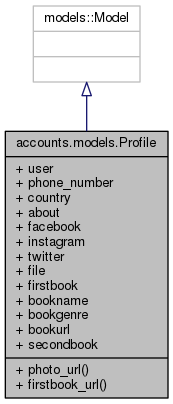
\includegraphics[scale=.85]{images/classaccounts.png}
    \caption{Class Diagram for accounts.models.Profile}
    \label{fig:collaborative1}
\end{figure}

\begin{figure}
    \centering
    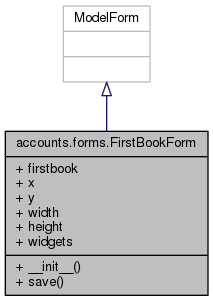
\includegraphics[scale=.85]{images/classacountsform.png}
    \caption{Class Diagram for accounts.forms.FirstBookForm}
    \label{fig:collaborative}
\end{figure}

\begin{figure}
\centering
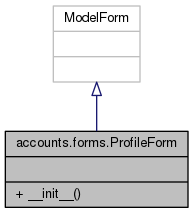
\includegraphics[scale=.85]{images/profileform.png}
\caption{Class Diagram for accounts.forms.ProfileForm}
\label{fig:classAnnotation__coll__graph}
\end{figure}
